%&latex
\documentclass[a4paper]{report}
\usepackage{commons/commons}
\usepackage{commons/note_style}

\usepackage{comment}
\usepackage{titlesec}
\titleformat{\chapter}[display]
  {\normalfont\sffamily\big\bfseries\color{black}}
  {\chaptertitlename\ \thechapter}{5pt}{\huge}
%\excludecomment{figure}

\def\ojoin{\setbox0=\hbox{$\bowtie$}%
  \rule[-.02ex]{.25em}{.4pt}\llap{\rule[\ht0]{.25em}{.4pt}}}
\def\leftouterjoin{\mathbin{\ojoin\mkern-5.8mu\bowtie}}
\def\rightouterjoin{\mathbin{\bowtie\mkern-5.8mu\ojoin}}
\def\fullouterjoin{\mathbin{\ojoin\mkern-5.8mu\bowtie\mkern-5.8mu\ojoin}}
\usepackage{amsbsy}
\usepackage{amstext}
\begin{document}

%+Title
\title{Advanced Database Quicksheet}
\author{Daniel D. Zhang}
\date{Fall 2015. \today}
\maketitle
%-Title

%+Abstract
%\begin{abstract}
%This is the notes for CSE 232A.
%\end{abstract}
%-Abstract

%+Contents
\tableofcontents
%-Contents
\chapter*{Preface}
\section*{Preclude}
\begin{itemize}
\item \textbf{NULL}: NULL means absence of value. Any value \textbf{cannot} ever be $=$ (or $<>$) NULL because NULL has no value. However, SQL has special IS NULL and IS NOT NULL predicates for dealing with NULL.
\end{itemize}
\section*{Acronyms}
\
\begin{obeylines}
\rih{Attr}. Attributes 
\rih{Ptr}. Pointer
\rih{Mgt}. Management 
\rih{idx}. Access key to array, that is array index; but it is not the database index.

\end{obeylines}
\chapter{Introduction}
\begin{itemize}
\item Basic SQLs 
\item \rih{ACID}: Atomicity, Consistency, Isolation, Durability 
\begin{enumerate}
\item Atomicity: each transaction be "all or nothing".
\item Consistency: any transaction will bring the database from one valid state to
another.
\item Isolation: the concurrent execution of transactions results in a system state
that would be obtained if transactions were executed serially
\item Durability: once a transaction has been committed, it will remain so, even in
the event of power loss, crashes, or 
\end{enumerate}
\item Transaction Mgt
\item Database System Architecture. Fig:
\begin{figure}[hbtp]
\centering
\subfloat{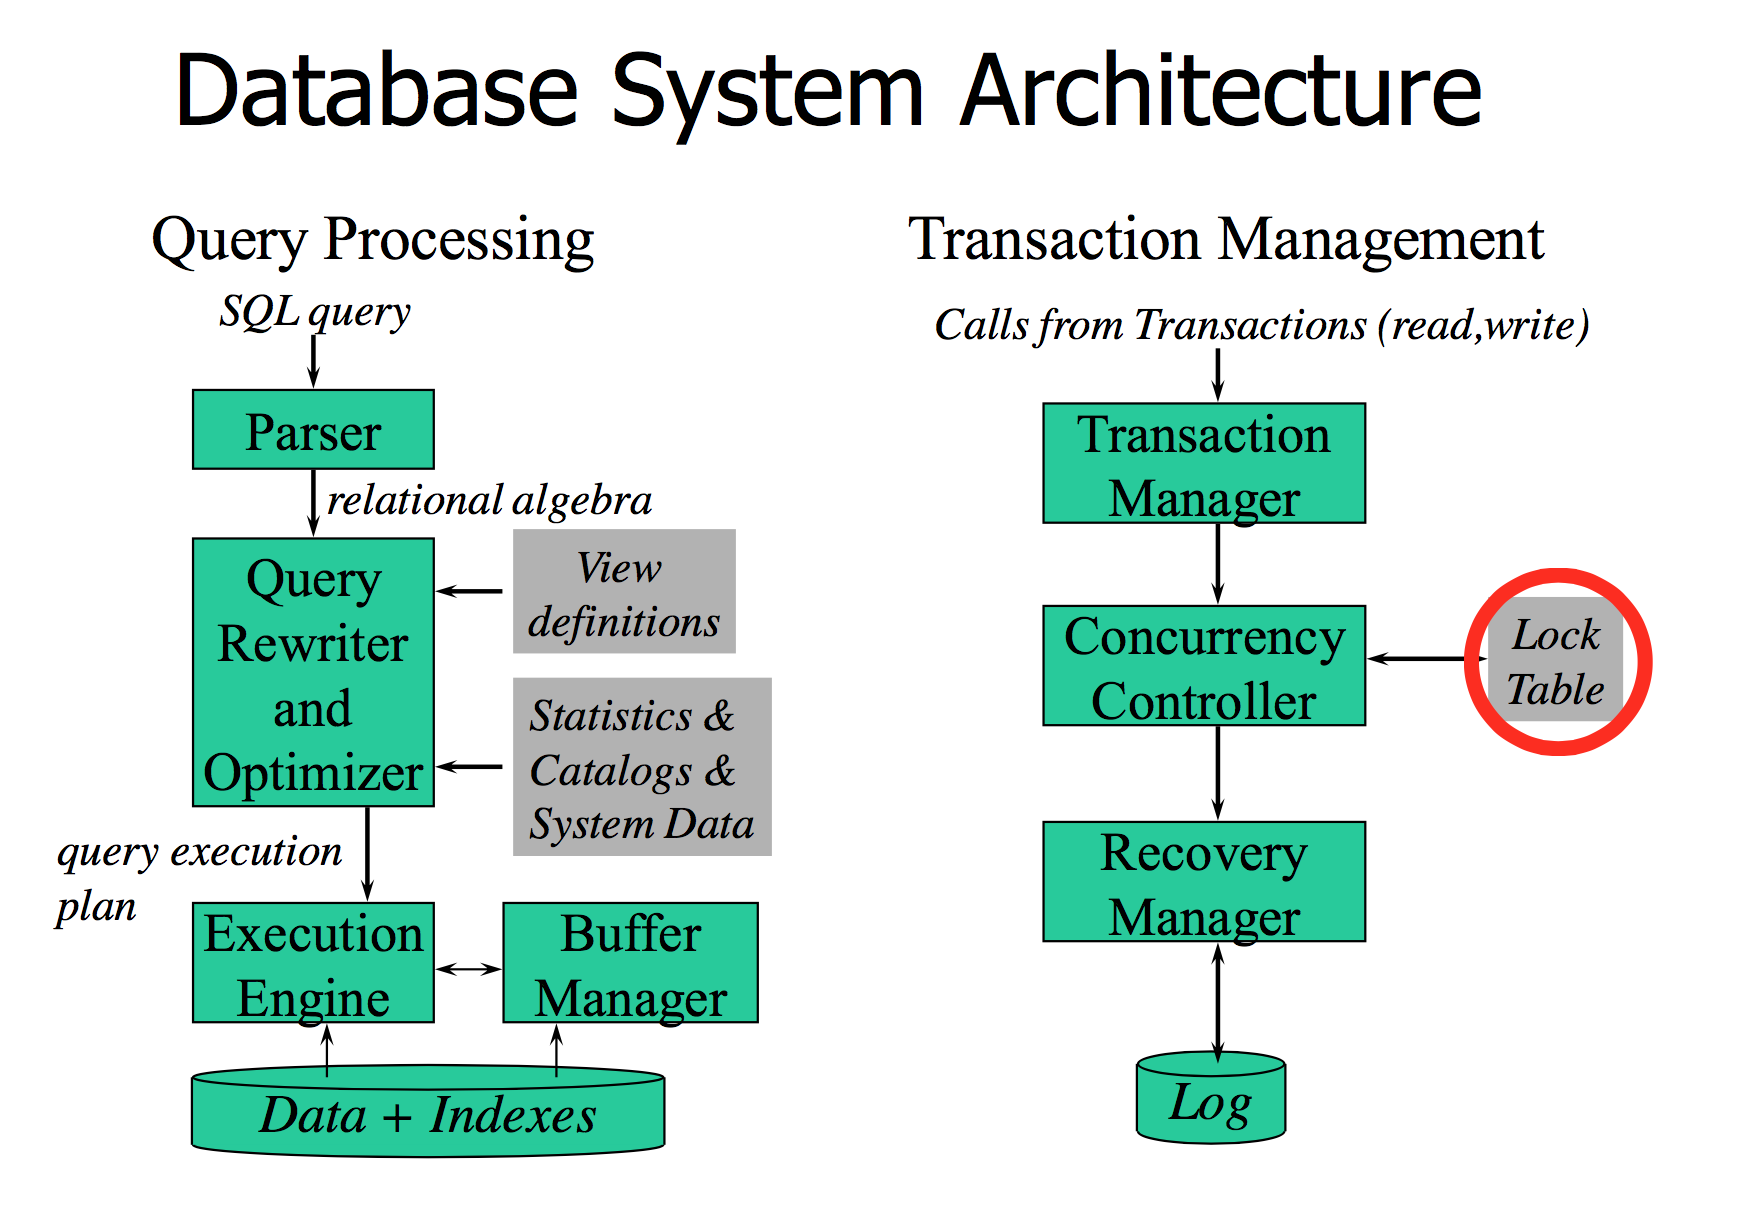
\includegraphics[height=2.2in]{img/db_sys_arch}}
\caption{Database System Architecture}
\label{fig:LABEL}
\end{figure}
\end{itemize}


\chapter{Hardware}
\begin{itemize}
\item Memory Hierarchy 
\begin{enumerate}
\item Blocked-based access 
\item Different Rates of Improvement 
\end{enumerate}
\item Tuned for blocks: Two-Phase, Multiway MergeSort (TPMMS). 
\begin{enumerate}
\item Phase 1: Load and sort into multiple lists 
\item Phase 2: Merge multiple lists 

Upper data size: 
$$
\frac{M^2}{B}
$$
, where $M\trieq$ RAM byte size, $B\trieq$ block byte size (rather than \#blocks).

core clues, TODO

Block I/O cost:
\begin{enumerate}
\item phase 1: B(R) read + B(R) write 
\item phase 2: B(R) read + B(R) write 
\end{enumerate}
, where B(x) is the number of block. 
\end{enumerate}
\end{itemize}


\chapter{Indexing}
\section{Conventional indexes}
\begin{enumerate}
\item Basic index types
  \begin{enumerate}
  \item Primary index
  \item Secondary index. 

  Notice the order of index: $i+1, i$ level of indexes. Secondary is meaningless to have a dense index. 
  
  
  
  \end{enumerate}
  \begin{enumerate}
  \item Dense Index
  \item Spare Index
  \end{enumerate}
\item Multi-level indexes
\item Operations on conventional index
  \begin{enumerate}
  \item Duplication
  \item Deletion
  \item Insertion
  \end{enumerate}
\item Secondary Indexes
  \begin{enumerate}
  \item Non-sequencing \& multi-level
  \item Duplicate values
  
  Solutions:
    \begin{enumerate}
    \item Multiple index ptrs
    \item variable size of index list 
    \item chaining records 
    \item bucket (most used)
    \end{enumerate}
  \end{enumerate}
\end{enumerate}
\section{B+Tree}
\subsection{Basics}
Root node can be any size. 

\begin{tabular}{lll}
\hline\noalign{\smallskip}
\textbf{Attrs} & \textbf{Non-leaf} & \textbf{Leaf} \\
\noalign{\smallskip}\hline\noalign{\smallskip}
Ptrs & \lceil\frac{n+1}{2}\rceil & \lfloor\frac{n+1}{2}\rfloor \\
\noalign{\smallskip}\hline\noalign{
\caption{Non-root bodes at least half-full}
\end{tabular}

\begin{itemize}
\item Follow the range convention of $[a, b)$.
\item Left leaning convention 
\end{itemize}

\subsection{Operations}
Core clues
\begin{enumerate}
\item \textbf{Invariant}: children balanced or left-leaning
\item \textbf{Split}: split half, thus invariant.
\item \textbf{Leaf-Up}: no delete, recursively move up the right node's first child; thus invariant.
\item \textbf{Nonleaf-Up}: delete and recursively move up the left's last if left-leaning or right's first if balanced; thus invariant. 
\end{enumerate}

\section{Hash}
\subsection{Extensible hashing}
Core clues:
\begin{enumerate}
\item Number of \textit{higher} order bit used $i$: $hash[:i]$ - \textbf{110}001
\item When overflow:
  \begin{enumerate}
  \item \textbf{Expand} the index $i=i+1$.
  \item \textbf{Split} the bucket. Reorganized the split bucket according to new $i$.
  \item \textbf{Untouched} buckets remain untouched. 
  \end{enumerate}
\item Shorthand notation: 110 \framebox{3} K I
\end{enumerate}
\begin{figure}[H]
        \centerline{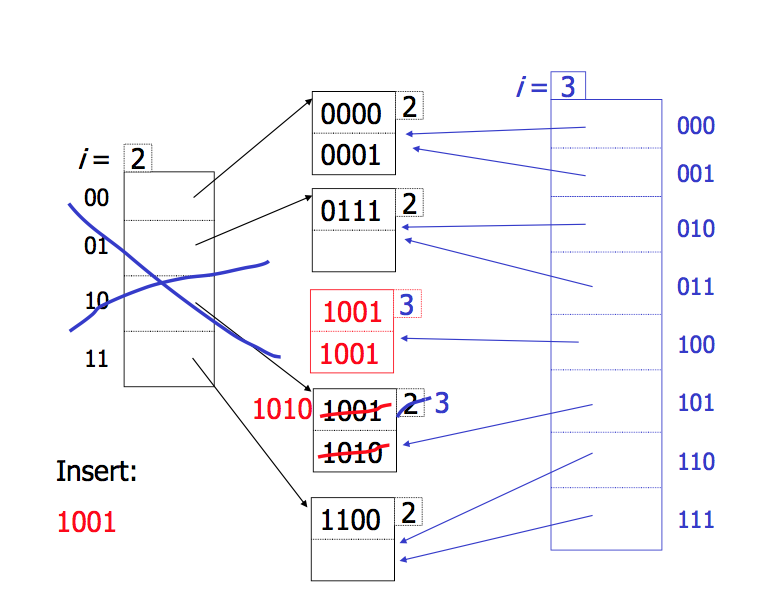
\includegraphics[height = 2in]{img/extensible_hashing}}
        \caption{Piazza}
    \label{fig:extensibleHashing}
\end{figure}
\subsection{Linear Hashing}
\begin{figure}[H]
        \centerline{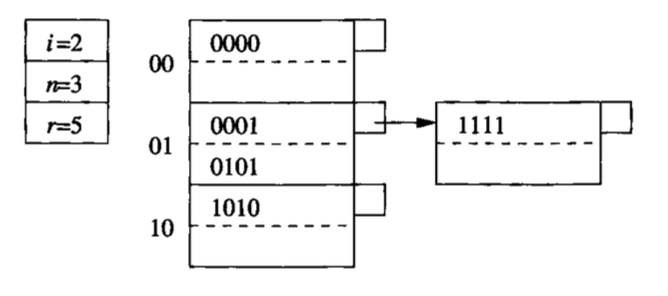
\includegraphics[height = 1in]{img/linearhashing}}
        \caption{Linear Hashing}
    \label{fig:linearHashing}
\end{figure}
Definitions:
\begin{itemize}
\item $m \triangleq a_1a_2...a_i$, the $i$ \textit{lower} bits of $H(K)$ intended for hashing - 110\textbf{001}
\item $n$ number of buckets (blocks) currently using (max number); doesn't count overflow block. 
\item $r$ number of records
\item $\tau$ threshold for $\frac{r}{n*cap}$, where $cap$ is the number of slots per block (textbook is $\frac{r}{n}$).
\end{itemize}
Insert: 
\begin{itemize}
\item if $m<n$, insert at $m$-th bucket.
\item if $n\leq m < 2^i$, insert at $0a_2...a_i$-th bucket, (unset the \textit{highest} bit of usage bit $m$).
\item if designated bucket full, append overflow block. 
\end{itemize}
Expand:
\begin{itemize}
\item if $\frac{r}{n*cap}>\tau$, inc $n$ $\wedge$ if the bucket idx is like $1.*$, split the corresponding $0...$ bucket. 
\item if $n>2^i$, inc $i$. Bucket idx remain unchanged. ($i$ can be derived from $n$) 
\end{itemize}

\section{BitMap}
\begin{figure}[H]
\centering
\subfloat{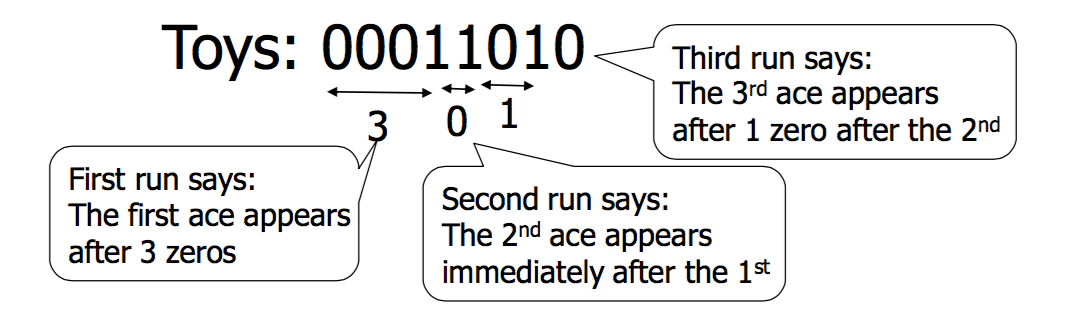
\includegraphics[scale=.80]{img/bitmap}}
\caption{Bitmap}
\label{fig:LABEL}
\end{figure}
Core clues:
\begin{enumerate}
\item Gap count of 0's between 1's
\item Encode length information [1]*(i-1)+[0], where i is number of bit for the gap count.
\item Checksum: len info and gap count are of same size
\end{enumerate}
Complexity: 
\begin{align*}
& \sim m \frac{n}{m} 2\log\Big(n/\frac{n}{m} \Big) \\
& \sim n \cdot 2\log m 
\end{align*}
Derivations:
\begin{itemize}
\item $n = T(R)$, $m = V(R, A)$
\item Assume 1's evenly distributed 
\item $\frac{n}{m}$ 1's for each bitmap (i.e. $\frac{\#1's}{unc\ bitmap}$).
\item For an unc bitmap: n-bit length with $\frac{n}{m}$ 1's; $\ra$ run is $\frac{n}{n/m}=m$, (precisely should consider the space taken by 1's)
\item For a comp bitmap: $\frac{n}{m}$ 1's with each run $m$, thus encoding length : $\frac{n}{m} 2 \log m$
\item Thus, in total: $m \cdot \frac{n}{m} \cdot 2 \log{m} = 2n\log m$
\end{itemize}

To summarize: 
$$
\#bitmaps \cdot \#1's\in bitmap_i \cdot 2\log\Big(\overline{gapLen\in 0's}\Big)
$$


\chapter{Query Processing}
\section{Basic query processing}
\subsection{Relational algebra}\label{rlsAlgebra}
Notations:
\begin{enumerate}
\item $\sigma$: Selection, WHERE (conditions). Selection does not preserver index.
\item $\times$: Cartesian product, FROM product. It does not de-dup columns.  
\item $\Pi$: Projection, SELECT (attributes)
\item $x\ra y$: Extended projection, rename $x$ to $y$. Scalar func: $a+b\ra y$, String ops: $c||d \ra y$

\textbf{Scalar} functions: their input comes from the same tuple (as opp. \textbf{aggregate})
$$
\Pi_{x, y\ra z, x+y\ra w} R
$$
Alternatively, $PLUS_{x, y\ra z}$; similarly $CONCAT, MULT, CONCAT}$
\item $\bowtie$: Natural join: $R\bowtie S = \Pi_{distinctAttrs}\sigma_{condOnBoth}(R\times S)$. Notice that the $\times$ is \textbf{bag} version; and $\bowtie$ de-dups columns. The results $LHS\equiv RHS$, but the query plans of $LHS, RHS$ may be different. 

\item $\bowtie_{\theta}$: $= \sigma_{\theta} (R\times S)$. $\theta$ is a condition. Notice that, $\bowtie_\theta$ is \textit{not} the $\theta$ version of natural join, but the $\theta$ version of Cartesian product. It does \textit{not} de-dup columns. 
\item $\gamma$: Group and aggregation

\textbf{Aggregate} functions. 
$$
\gamma_{attr_{grpby}, aggrFn(attr) \ra attr'}
$$
Alternatively, $SUM_{attr_{grpby},aggrFn(attr)\ra attr'}$, similarly $AVG, MIN, MAX, COUNT$.
\item $\tau$: Order by. 

A result $o(exp)$ is ordered if
\begin{enumerate}
\item $o$ retains the originally ordered $exp$. (e.g. $\sigma$)
\item $o$ creates ordering. (e.g. ordered by pk, then iterative joining implt with FLY)
\end{enumerate}
$\sigma$ may retain the order generated by $\tau$ but depends on implementation. e.g. $\sigma^\text{FLY}$ may prodeces a ordered result. Discussion: 

$$
\tau_{R.A, R.B}\ \sigma_{R.B>5}^\text{FLY} R
$$
\begin{flushright}, produces a list\end{flushright}
$$
\sigma^\text{FLY}_{R.B>5}\ \tau_{R.A, R.B} R 
$$
\begin{flushright}, produces a bag but preserves the order.\end{flushright} 
\end{enumerate}
\subsection{Query Plan}
A simple SFW (Select From Where). 
\begin{enumerate}
\item Naive plan p:
$$
\Pi_{attr_1,attr_2}^\text{FLY}\Big[\sigma_{cond_R\wedge cond_S\wedge cond_{RS}}^\text{FLY} (R^\text{SCAN}\times S^\text{SCAN})\Big]
$$

FLY and SCAN are how exactly the plan is run.
\begin{enumerate}
\item \textbf{FLY}: on the fly, one entry at a time. Implementation: Iterator. No intermediate storage 
\item \textbf{SCAN}: scan the tables, one block at a time.
\begin{enumerate}
\item \textbf{Table-scan}. operator simply reads each block holding tuples of the relation.
\item \textbf{Index-scan}. uses an index to find tuples
\item \textbf{Sort-scan}. produces the tuples in sorted order.

\end{enumerate}}
\end{enumerate}

\item Join Plan (plan II):
$$
\Pi_{attrs} \Big[(\sigma_{cond_R}R)  \bowtie^\text{HASH} (\sigma_{cond_S}S) \Big]
$$
\item Index plan (plan III):

$$
\Pi_{attrs}\ \sigma_{cond_S}(\sigma_{cond_R}^\text{INDEX}R \bowtie^\text{RI} S)
$$
$\bowtie^\text{RI}$ Right Index Join. 
Steps:
\begin{itemize}
\item $\sigma$ uses index to get tuples based on condition on $R$. 
\item $\bowtie^\text{RI}$. For each tuple in the result $R$:
\begin{itemize}
\item Match $S$'s tuple using $S$'s index, in $O(1)$. 
\end{itemize}
\item $\sigma$ filters $S$ based on condition on $S$.
\item $\Pi_{attrs}$ ...
\end{itemize}
\end{enumerate}
\section{From query to optimal plan}
\begin{enumerate}
\item \textbf{lqp}. logical query plan $\equiv$ algebra ops 
\item Algebraic rewritings to transform the lqp
\item Physical Plan
\item Example:
\begin{itemize}
\item \textbf{``In'' Elimination}: 
\begin{lstlisting}
SELECT A.a
FROM A WHERE A.v IN (
    SELECT B.v
    FROM B
    WHERE cond_b
);
\end{lstlisting}
IN is transformed into $\sigma (A\times B)$. Then the basic algebra is:
$$
\Pi_{A.a}\ \sigma_{A.v=B.v}\quad (A \times \Pi \sigma B)
$$
Further optimized:
$$
\Pi_{A.a}(A \underset{A.v=B.v}\bowtie \Pi \sigma B)
$$

\end{itemize}
\end{enumerate}
\section{Bag algebra, list algebra, and extensions}
In this nodes, bag-version operations are assumed. 
\begin{enumerate}
\item Algebraic Operators (Bag Version) $\cup, \cap$
$$
R\cup S
$$
\item Convert to set (DISTINCT)
$$
\delta(R)
$$
\item Extended relational algebra - Section \ref{rlsAlgebra}.
\end{enumerate}
\section{Relational algebra optimization}
\subsection{Rewriting}
\begin{enumerate}
\item \rih{Commutativity and Associativity}
\begin{align*}
R \cdot S &= S\cdot R \\
R\cdot (S\cdot T) &= (R\cdot S) \cdot T \\
\end{align}

, where $\cdot \in \{\times, \bowtie, \cup, \cap \}$  

proof: $R\times S = S\times R$
\begin{align*}
& R \times S \subset S \times R \\
& R \times S \supset S \times R \\
& \forall t, t\in R\times S,\mbox{ n times} \\
& r \in R\mbox{ m times}, s\in S \mbox{ k times}\\
& n = m*k \\
& \Ra\mbox{ find corresponding }t \in sr, k*m,\mbox{ n times} \\ 
& \therefore R \times S \subset S \times R \\
& \mbox{vice versa...}
\end{align*}
\item \rih{Logics}
\begin{align*}
\sigma_{cond_1\wedge cond_2}R &= \sigma_{cond_1}\ \sigma_{cond_2}R \\
\sigma_{cond_1\vee cond_2}R &= \sigma_{cond_1}R \cup \sigma_{cond_2}R
\end{align*}

\begin{flushright}, notice that $\vee$ only applies for set-version\end{flushright}

Decomposition of Negation:
TODO

\item \rih{Push down $\sigma$} !important
\begin{itemize}
\item General
$$
\sigma_{cond}(R\cdot S) = (\sigma_{cond} R)\cdot (\sigma_{cond} S) 
$$
\begin{flushright}, where $\cdot\in \{-, \cup, \times, \bowtie\}$. \end{flushright}

\item For $\{-\}$, it can directly drop the selection: $\sigma_{cond}S$ to $S$. 
$$
\sigma_{cond}(R-S) = (\sigma_{cond} R)-S
$$
\item For $\{\times, \bowtie\}$, it can further drops the $\sigma_{cond}T$ to $T$ if the condition does not refer to attributes in $T$.
\begin{align*}
\sigma_{cond}(R\cdot S) = R\cdot (\sigma_{cond} S) 
\end{align*}
\end{itemize}

proof: $\sigma_{A=2}(R\bowtie S) = (\sigma_{A=2}R)\bowtie S$, given commutativity and $\sigma_{cond}(R\bowtie S) = R\bowtie \sigma_{cond}S$
\begin{align*}
\sigma_{A=2}(R\bowtie S) = \sigma_{A=2}(S\bowtie R) = S \bowtie (\sigma_{A=2}R)=(\sigma_{A=2}R\bowtie S)
\end{align*}
This is a technique of proof by using axioms. 

\rih{Combine $\pi$ \& $\sigma$}

\item \rih{Push down $\pi$} 
 
\begin{align*}
& \pi_x (R \cup S) = \pi_x R \cup \pi_x S \\
& \pi_a (R \times S) = \pi_a (\pi_{cond1 \supseteq a}R \times \pi_{cond2 \supseteq a} S) \\
& \pi_a (R \bowtie S) = \pi_a(\pi_{cond1 \supseteq (a \cup R.c)}\ R \bowtie \pi_{cond2 \supseteq (a\cup S.c)}\ S) \\
& \pi_x R = \pi_x \pi_{y\supseteq x} R
\end{align*}
$\pi$ can reduce the length of a tuple; thus it is useful to push down $\pi$ to fit more tuples in memory. When denoting $\supset, \supseteq, \subset, \subseteq$, it is for AND composite. $cond1\supseteq a$ is a shorthand notation for $\{cond1|cond1 \supseteq a\}$, a notation for superset. 

\rih{Push down priority of $\pi, \sigma$}. Normally $\sigma$ is given higher priority than $\pi$ if $\sigma$ can do index selection to avoid $\pi$ on all tuples 
\item \rih{Aggregation} 

\begin{align*}
& \sigma_{cond\subset grpAttrs} \Sigma_{grpAttrs; attr\ra attr'} R = \Sigma_{grpAttrs, attr\ra attr'} \sigma_{cond\subset grpAttrs} R \\
& \Sigma_{GL;GA\ra RA} (R \cup S) = +_{RA1, RA2:RA} (\Sigma_{GL; GA\ra RA1 }R \bowtie \Sigma_{GL; GA\ra RA2} S)\\
& \Sigma_{GL2; RA1 \ra RA2} \Sigma_{GL1; GA \ra RA1} R = \Sigma_{GL2; GA\ra RA2} R
\end{align*}
Notation, in slides it is $grpList$ or $GL$ as $grpAttrs$; $SUM$ as $\Sigma$; $PLUS$ as +.
\item \rih{Cost, rule of thumb} 

\end{enumerate}
\subsection{Proof/Disproof the equivalence of rewriting}
The \note{breakthrough} points: 
\begin{enumerate}
\item $\phi$ table
\item NULL column. 
\end{enumerate}



\section{Algorithms for Relational Algebra Operators}
\subsection{Query Execution}
\subsubsection{Implementations of $\bowtie$}

Notice:
\begin{itemize}
\item Write out of the join result at the end is not considered due to pipeline.
\item Time of execution is measured by number of disk IO. 
\end{itemize}



\begin{enumerate}
\item Iteration join (one pass)

\textbf{Requirement}. $\min(B(R), B(S)) < M$

\textbf{Time}. Load a table to memory, and then loop join. Assumption $\min(B(R), B(S))<M$; thus
$$B(R)+B(S)$$
\item Merge join 

\textbf{Process.} Two phases:
\begin{enumerate}
\item Sort-merge phase. \textbf{Mem} req: $|R|/M<M; |S|/M<M$
\item Merge-join phase. \textbf{Mem} req: $|R|/M+|S|/M <M$
\end{enumerate}
Possible to combine the merge 

\textbf{Time.} 1 read 1 write for the sort, 1 read to the merge; thus 
\begin{align*}
3B(R)+3B(S) &\\
3B(R)+B(S) & \text{ if S is sorted on attr}
\end{align*}
\item Index join 

\textbf{Time.} when no relation fits in memory, $\bowtie^{RI}$ outperforms any other technique. It reads $B(R)$; for each $T(R)$, load $B(S)/V(S, B)$ blocks according to the index; thus 
\begin{align*}
B(R)+T(R)\cdot (1+\frac{B(S)}{V(S, B)}) &\text{ if R clustered}
% \\ T(R)+T(R)\cdot (1+B(S)/V(S, B)) &\text{ if R not clustered}
\end{align*}

\begin{itemize}
\item $1+...$, the 1 for \textit{index block access} to the non-cached leaf node of the B-tree index 
\item Create index (normally already created): read blocks and write index $B(S)+B(index)$
\end{itemize}
\item Hash join 

\textbf{Requirement.} $\min(B(R_{i}), B(S_{i}})) <M$. The smaller \textit{bucket} need to fit in mem when merge the bucket. 

\textbf{Process.} Two phases
\begin{enumerate}
\item Hash every tuple into $M-1$ buckets $R_i, S_i$ (the remaining 1 for the temp working memory).
\item Load either $R_i, S_i$ into mem, scan the other and join.
\end{enumerate}
\textbf{Time.} 1 read write R, S to create hashed buckets. 1 read to hash join; thus $$3B(R)+3B(S)$$
\end{enumerate}

\subsubsection{Analysis}
\begin{enumerate}
\item Results are \textit{pipelined}, thus not consider write the final result into disk. 
\item \textit{Sorted} table does not need to sort in sort-merge on the sorted attr.
\begin{enumerate}
\item 1-pass on sorted table, result may also be sorted (depends).
\item sort-merge will produce sorted result
\end{enumerate}
\item Intermediate results do not have index. 
\item calculate time $\leftarrow$ calculate the \# disk I/O $\leftarrow$ \# blocks $B(R)$ $\leftarrow$ intermediate tuple size $T(R)$. 
\end{enumerate}
\subsection{Cost analysis (intermediate size)}
\rih{Intro}
\begin{itemize}
\item Two aspects of cost analysis:
\begin{enumerate}
\item Size of the intermediate result 
\item Number of I/Os.
\end{enumerate}
\item Notations
\begin{enumerate}
\item T(R) : #tuples in R
\item S(R) : #bytes (size) in each R tuple
\item B(R): #blocks to hold all R tuples 
\item V(R, A) : #distinct values in R for attribute A
\end{enumerate}
\item Corner case 
$$
V(R_1\times R_2) \approx V(R_1, A)
$$
Corner case: $R_2=\phi$, then RHS should be 0. But, in size estimation, doesn't consider the corner case. Normally, only the average case (uniform distr.) is considered. 
\end{itemize}
\rih{Estimate for $\bowtie$}
\begin{itemize}
\item \textbraceleft PK, FK\textbraceright\ relationship $R_1\bowtie R_2$

One way PK, FK for $R_1, R_2$: 
$$
T(W) = \frac{T(R_1)}{V(R_1, A)} T(R_2)
$$

Generalized to symmetry: 
$$
T(W) = \frac{T(R_1)T(R_2)}{\max\{V(R_1, A), V(R_2, A)\}}
$$
\end{itemize}
\rih{Subexpressions \& Value preservation}

A probability approach. The combination should not change the a $V$'s prob distr. since assumped indpt.
\begin{itemize}
\item Value preservation for the pushing down of $\sigma$. 
\item Value preservation for the composite $\bowtie$. 
\end{itemize}
\subsection{Plan Enumeration}
\subsubsection{Hypergraph}
INGRES greedy heuristic search. 

%+Bibliography
\begin{thebibliography}{99}
\bibitem{Label1} ...
\bibitem{Label2} ...
\end{thebibliography}
%-Bibliography
\end{document}
